\documentclass[12pt]{article}

\usepackage{dsfont}
\usepackage{amsmath}
\usepackage{graphicx}
\usepackage[margin=1.00in]{geometry}

\usepackage{bm}
\newcommand{\m}[1]{\mathbf{\bm{#1}}}
\newcommand{\R}{I\hspace{-4.4pt}R}

\setlength\parindent{0pt}

\begin{document}

Mickey Warner
\bigskip

\subsection*{Introduction}

We fit a discrete process convolution model to the ozone in the Northeast. A Bezier kernel with varying range parameter is used. We consider as priors independent and identically distributed normals (model 1) and a Gaussian Markov random field (model 2) for the coefficients associated with the kernel. Instead of working with longitude and latitude as our coordinates, we work with northing and easting (assuming UTM grid zone 19). The models were fit at knots that made up a (roughly) evenly spaced grid in our region of interest.

\subsection*{Knots and data points}
Figure 1 shows the locations of the observed ozone measurements (blue) and the specification of the knots (orange). There are a total of 69 knots which surround the data. The knots go beyond the data in an attempt to handle any boundary effects. Some outliers and leverage points were removed.

\begin{figure}[ht]
\begin{center}
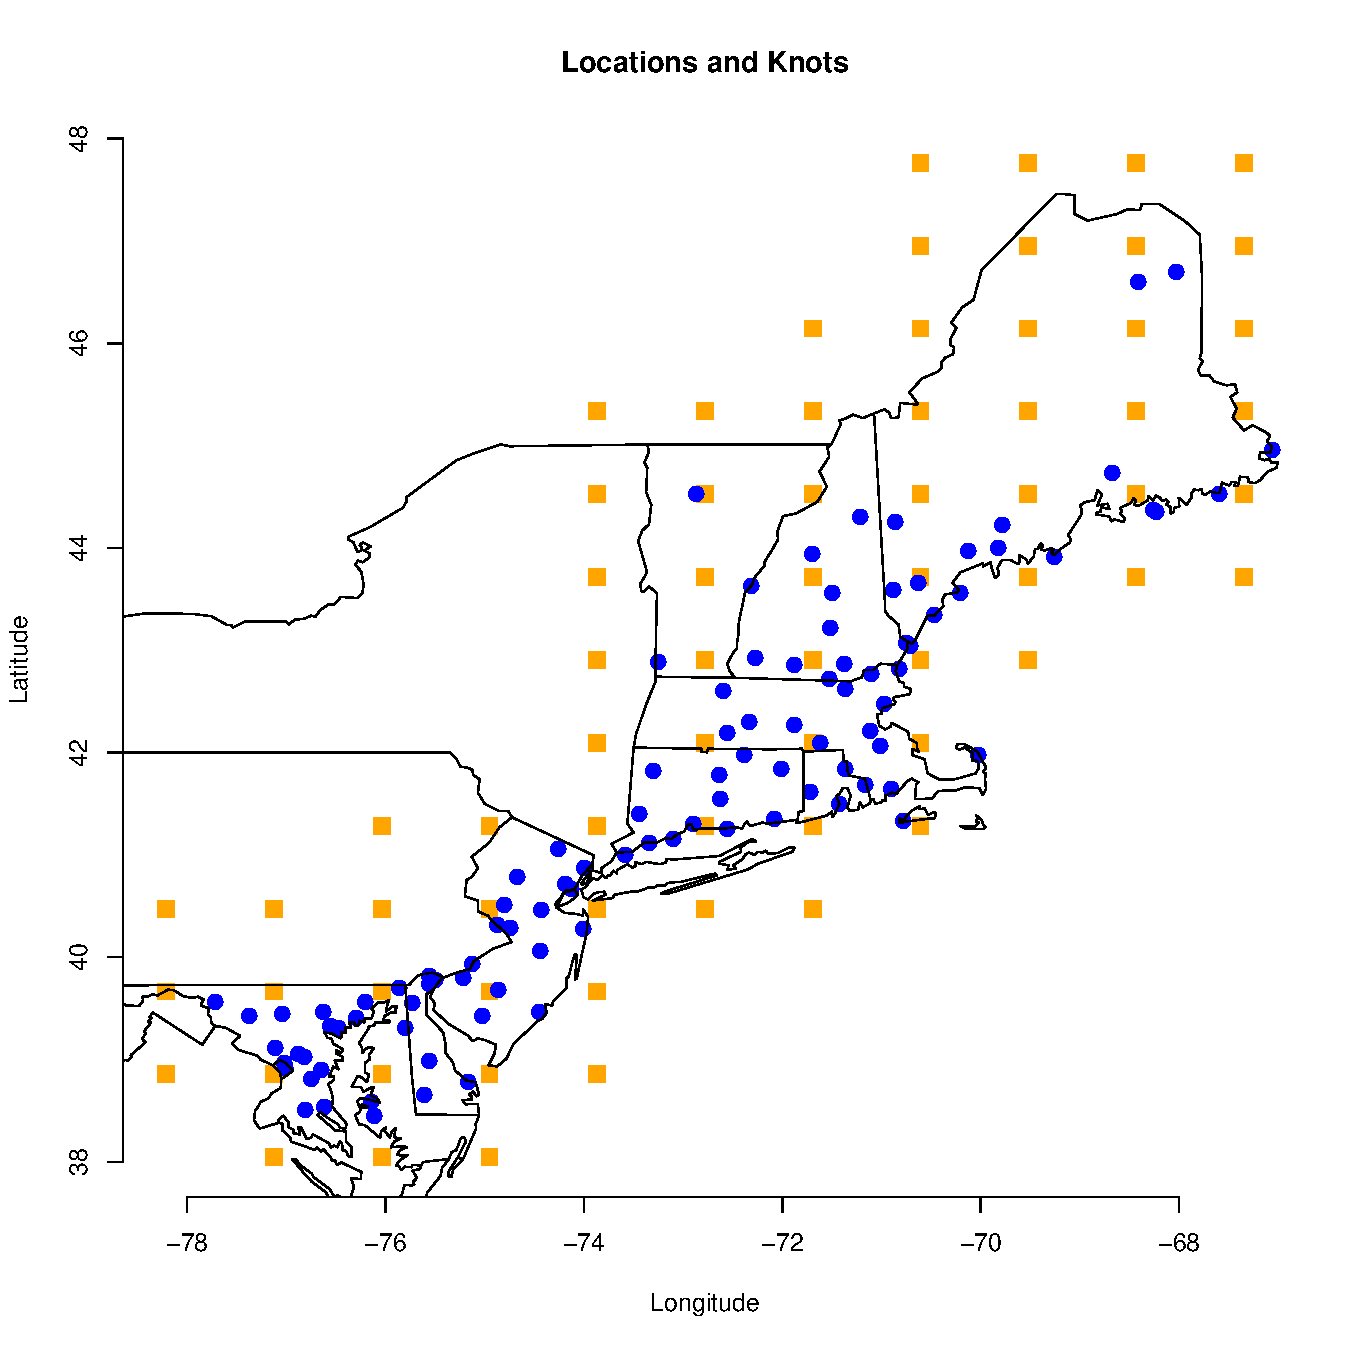
\includegraphics[scale=0.5]{figs/knots.pdf}
\end{center}
\caption{Blue points: all locations where ozone is observed. Orange points: the knots used to fit the models.}
\end{figure}

\subsection*{Discrete process convolution model}

At spatial locations $s_i$, the observed value $y_i$ is assumed to follow the discrete process convolution model

\[ y_i = \mu(s_i) + \sum_{j=1}^pk(s_i-u_j;\psi)w_j + \epsilon_i \]

where $\mu(s)=z(s)^\top\beta$ is the trend, $k(s-u;\psi)$ is the Bezier kernel, $w_j\overset{iid}\sim N(0,\sigma^2)$, and $\epsilon_i\overset{iid}\sim N(0,\tau^2)$. The knots $u$ are shown in Figure 1 as the orange squares. The Bezier kernel is defined as

\[ k(s-u;\psi) = (1 - ||s-u||^2/\phi)^\nu \]

with $\psi=(\phi,\nu)$, defined on $||s-u||<\sqrt{\phi}$. We a select a trend to have an intercept and a linear component for northing. Model 1 assumes the $w_j$'s are i.i.d. normal.
\bigskip

Model 2 considers a different prior on $\m{w}=(w_1,\ldots,w_p)^\top$, specifically
\[ \m{w} \sim N(\m{0}, \sigma^2 W^{-1}) \]
We construct $W$ based only on the nearest neighbors of each knot, resulting in linear dependence between the convolution coefficients

\[ W_{ij} = \begin{cases} n_i & i=j \\ -1 & i\sim j \\ 0 & o.w. \end{cases}, \]
where $n_i$ is the number of neighbors of $w_i$ and $i\sim j$ denotes $w_i$ and $w_j$ are neighbors. In our dataset, this leads to a precision matrix $W$ that is singular. Therefore, we add a small $(0.01)$ amount to each diagonal element in $W$.
\bigskip

\subsection*{Discussion}

Figures 2 through 4 show a comparison between models 1 and 2. In Figure 2 we show the coefficients to the convolution process. There is minimal overlap between the models in this regard. In model 1 we see estimates, on the whole, slightly smaller than in model 2. The same could be said for the standard deviation. As expected, model 2 does seem to do a better job at including spatial correlation between the knots.
\bigskip

The surfaces in Figure 3 and very nearly the same for both models. The major issue here is that we seem to be picking up only the trend in our predictions (northing). The convolution does not appear to make any contribution to our predictions. Figure 4 shows that there are clearly some observations we are not capturing (note those large observed values). Because of this, we do not believe our data is better fit to a trend only. Therefore, we would expect the kernel convolution to capture some of this uncertainty, but it is not.

\begin{figure}[ht]
\begin{center}
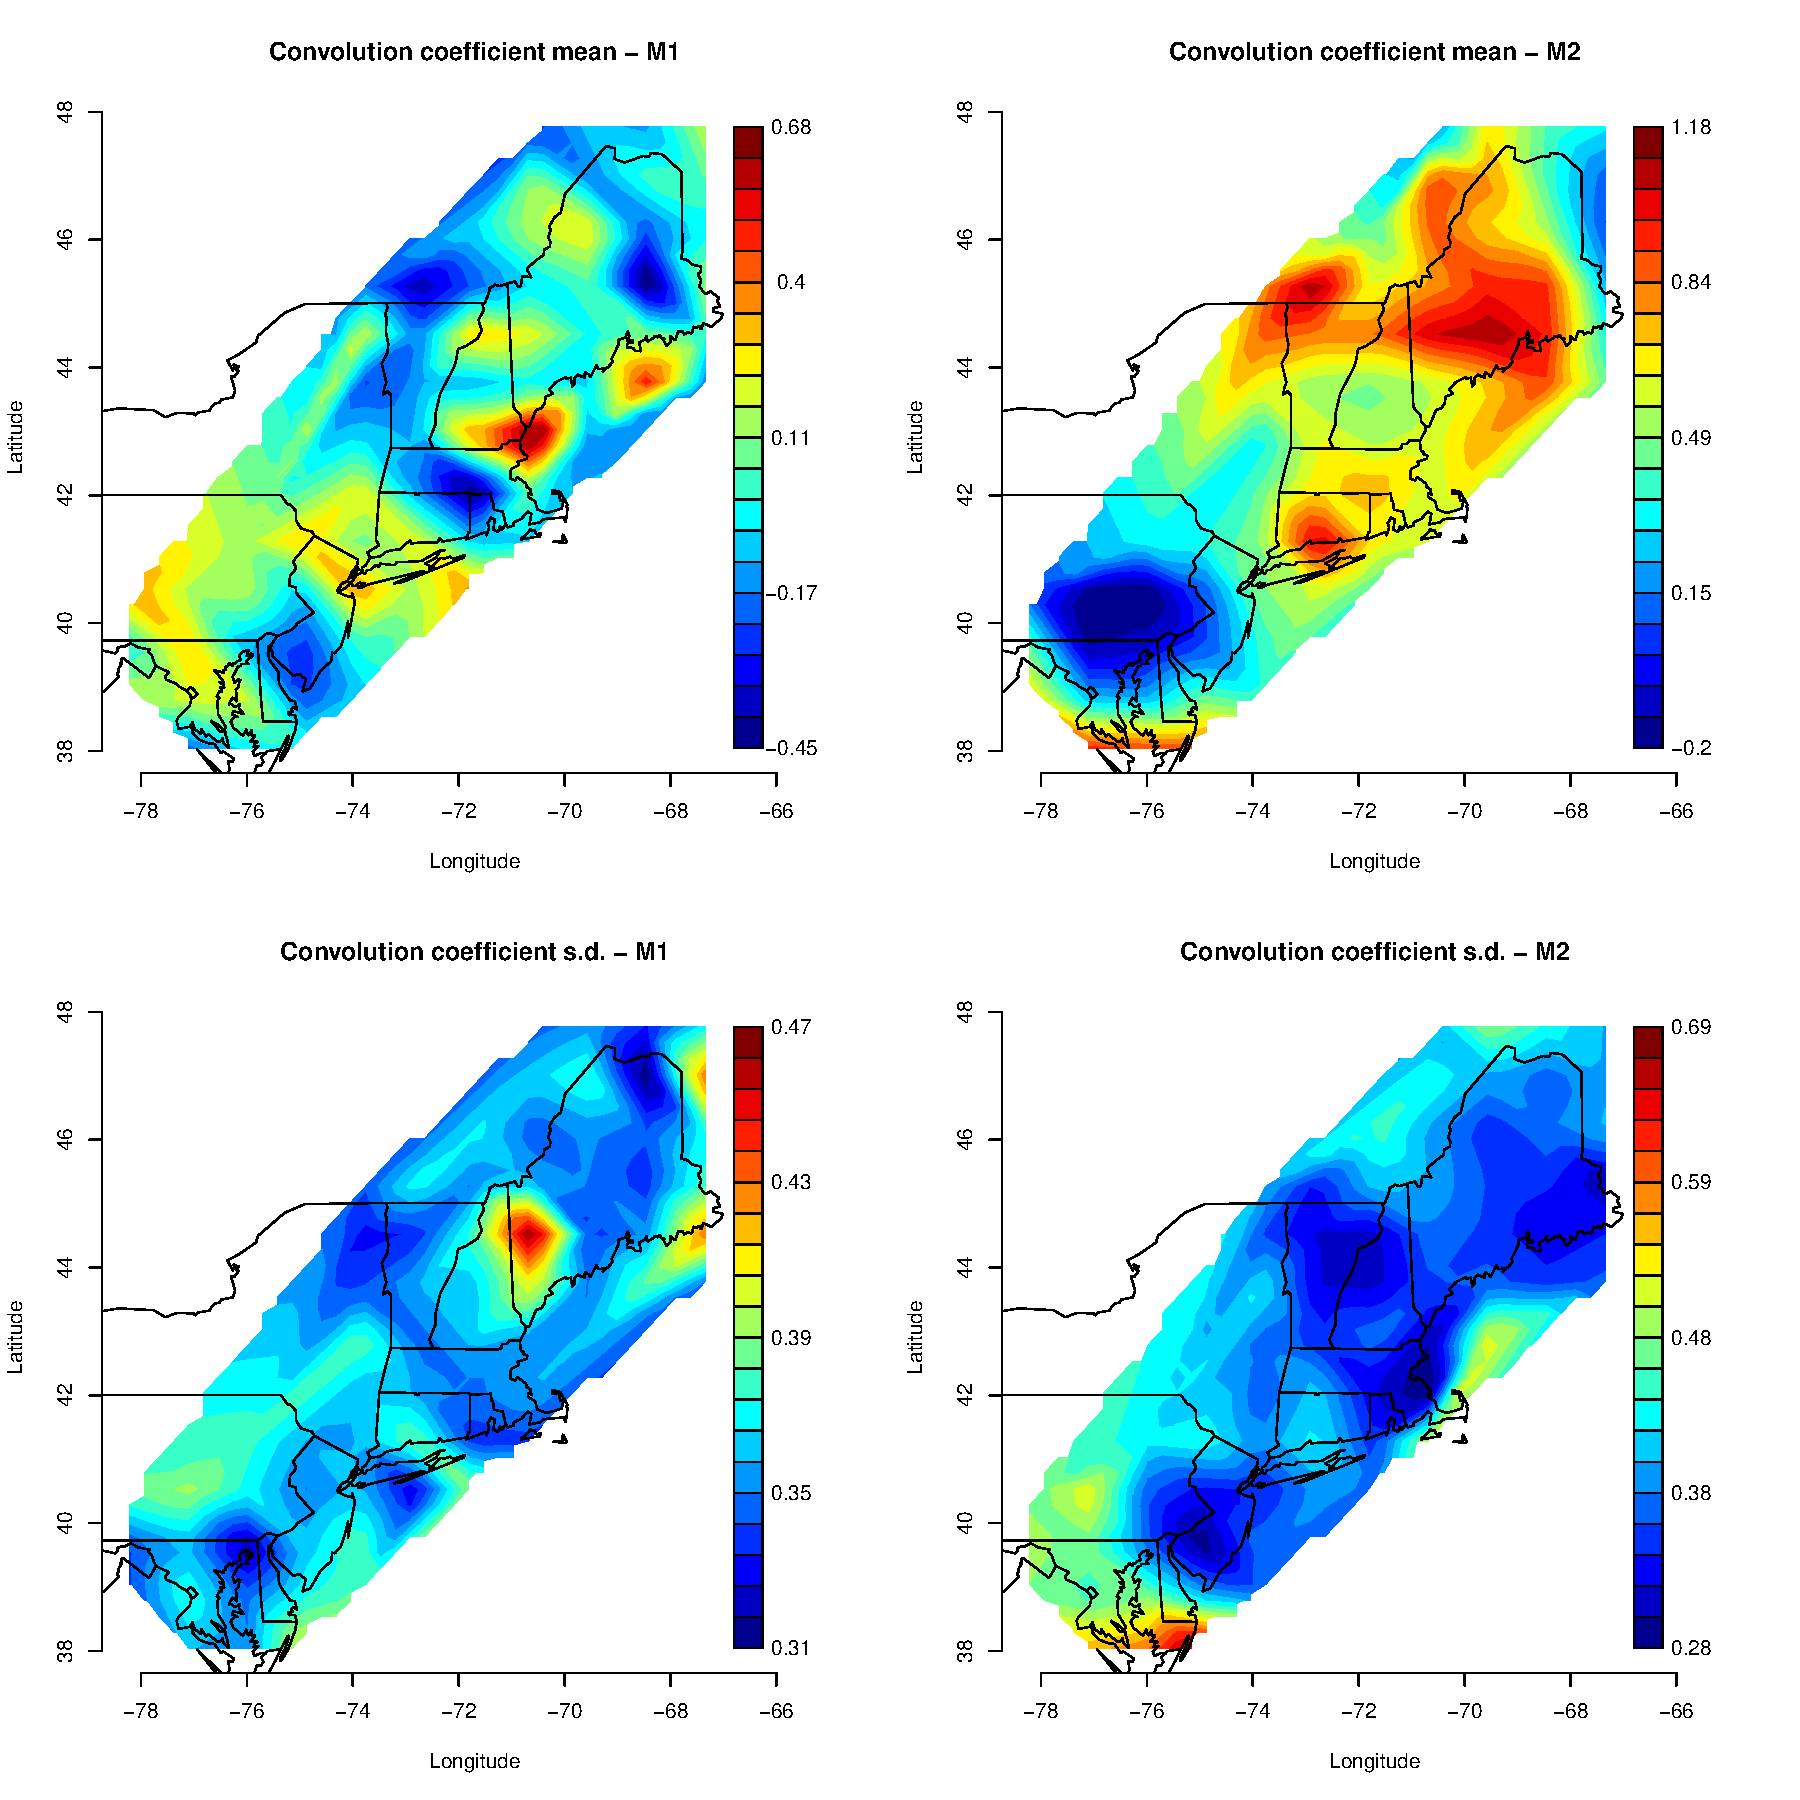
\includegraphics[scale=0.5]{figs/w.pdf}
\end{center}
\caption{Convolution coefficients. Top row: mean. Bottom: standard deviation. Left: model 1. Right: model 2.}
\end{figure}

% \begin{figure}[ht]
% \begin{center}
% 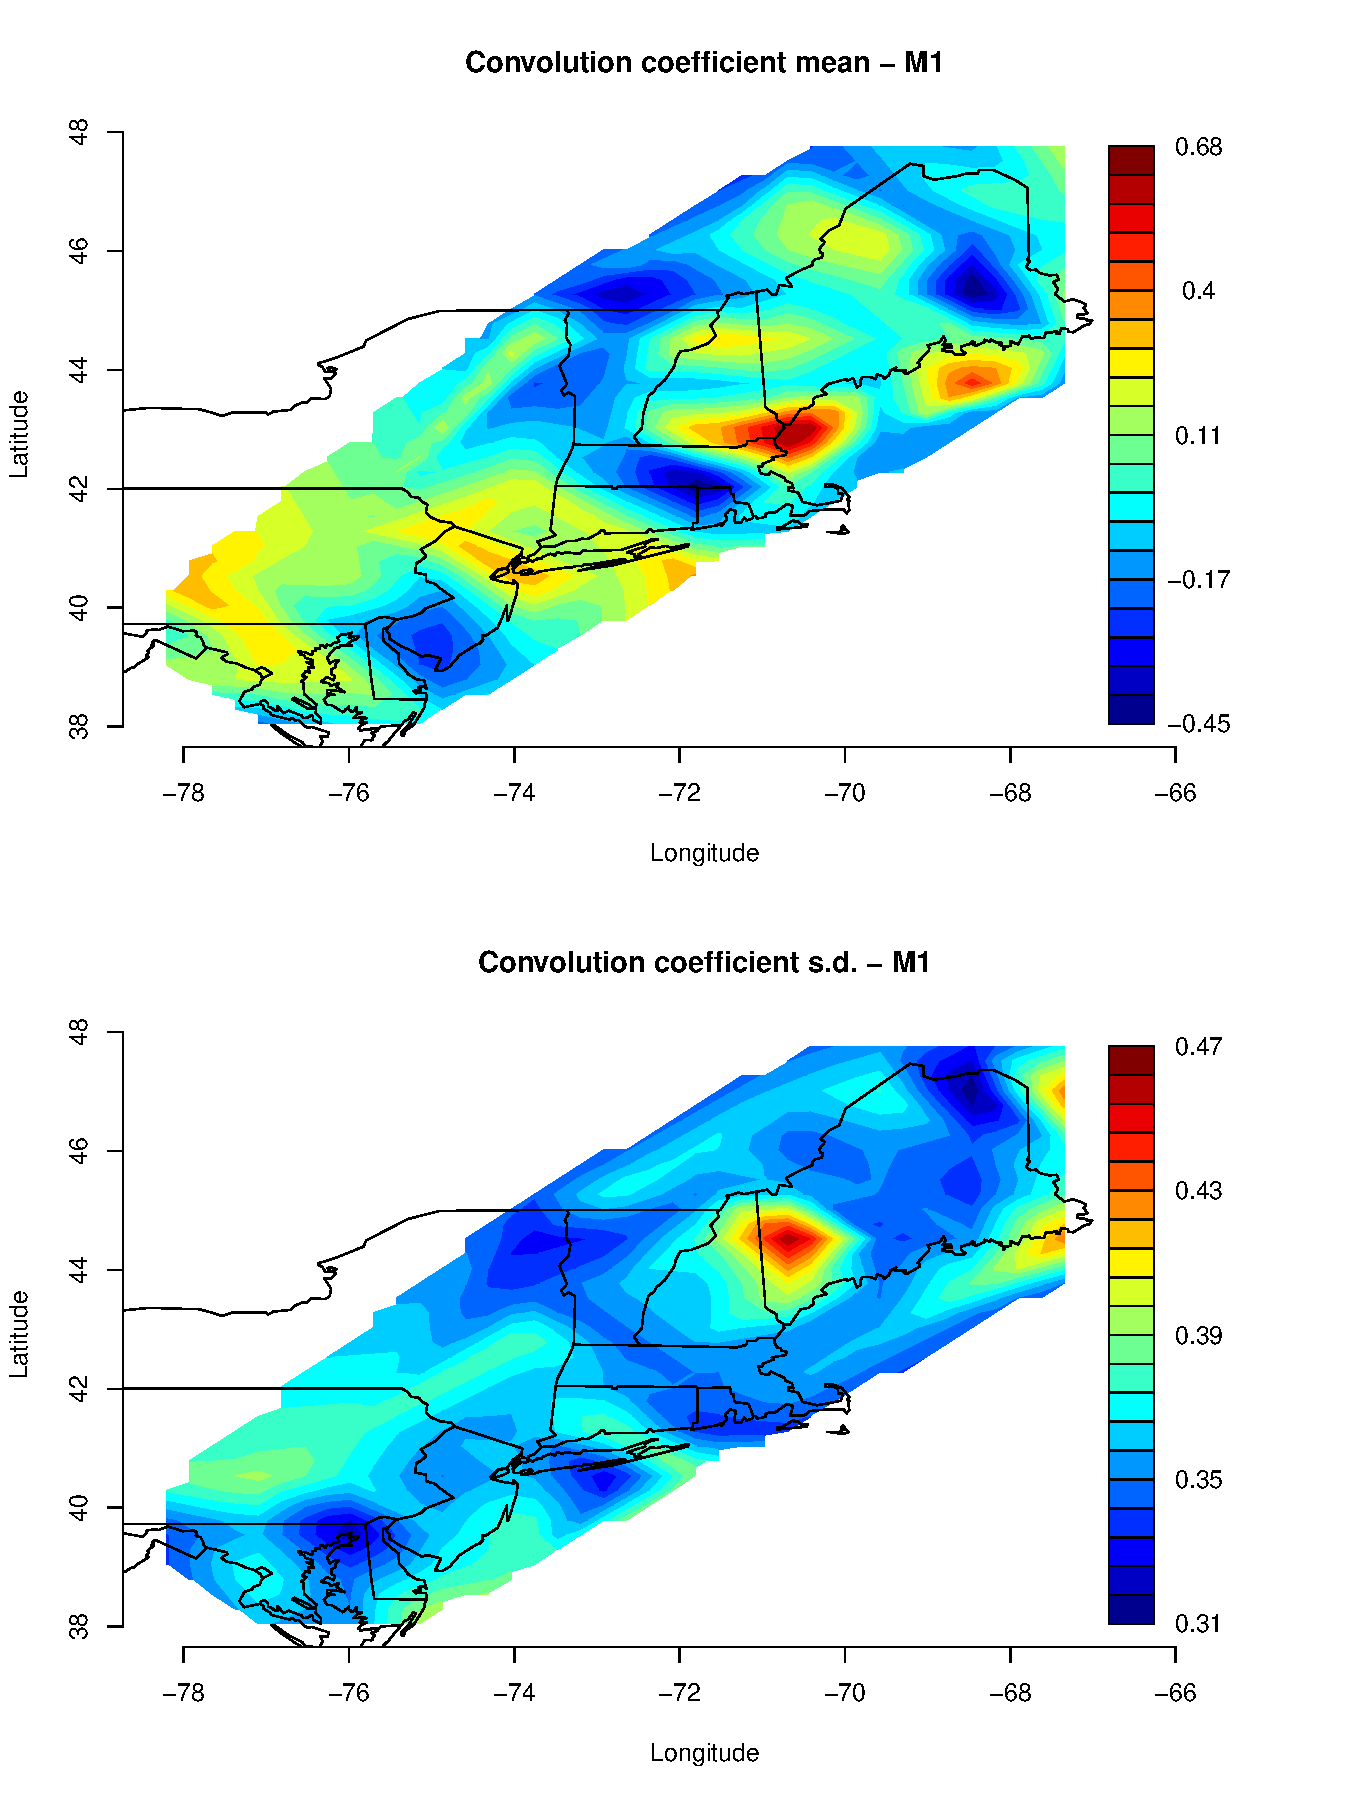
\includegraphics[scale=0.5]{figs/w1.pdf}
% \end{center}
% \caption{Convolution coefficients for model 1, i.i.d. normal prior}
% \end{figure}
% 
% \begin{figure}[ht]
% \begin{center}
% 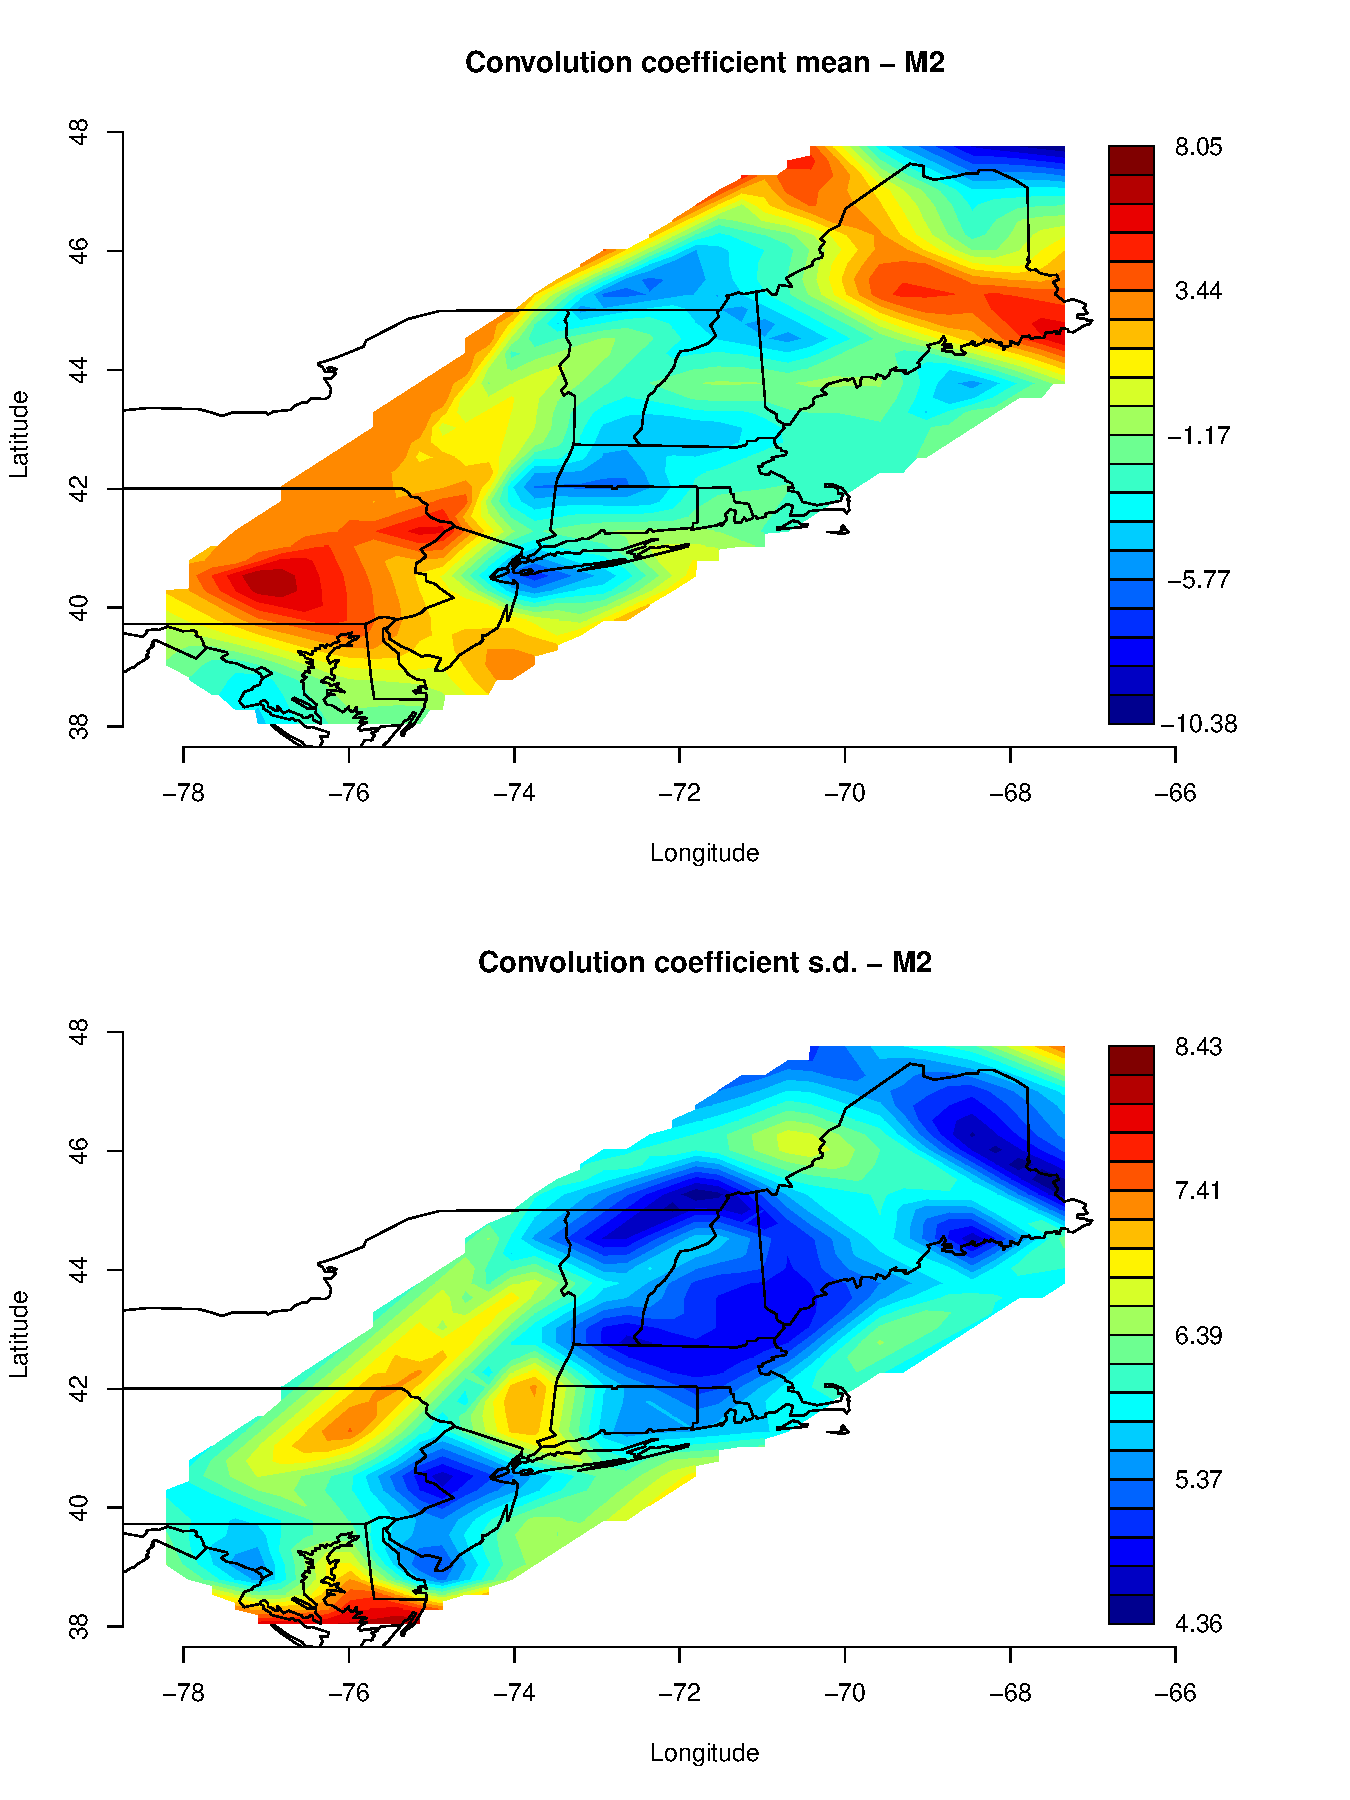
\includegraphics[scale=0.5]{figs/w2.pdf}
% \end{center}
% \caption{Convolution coefficients for model 2, nearest neighbor prior}
% \end{figure}

\begin{figure}[ht]
\begin{center}
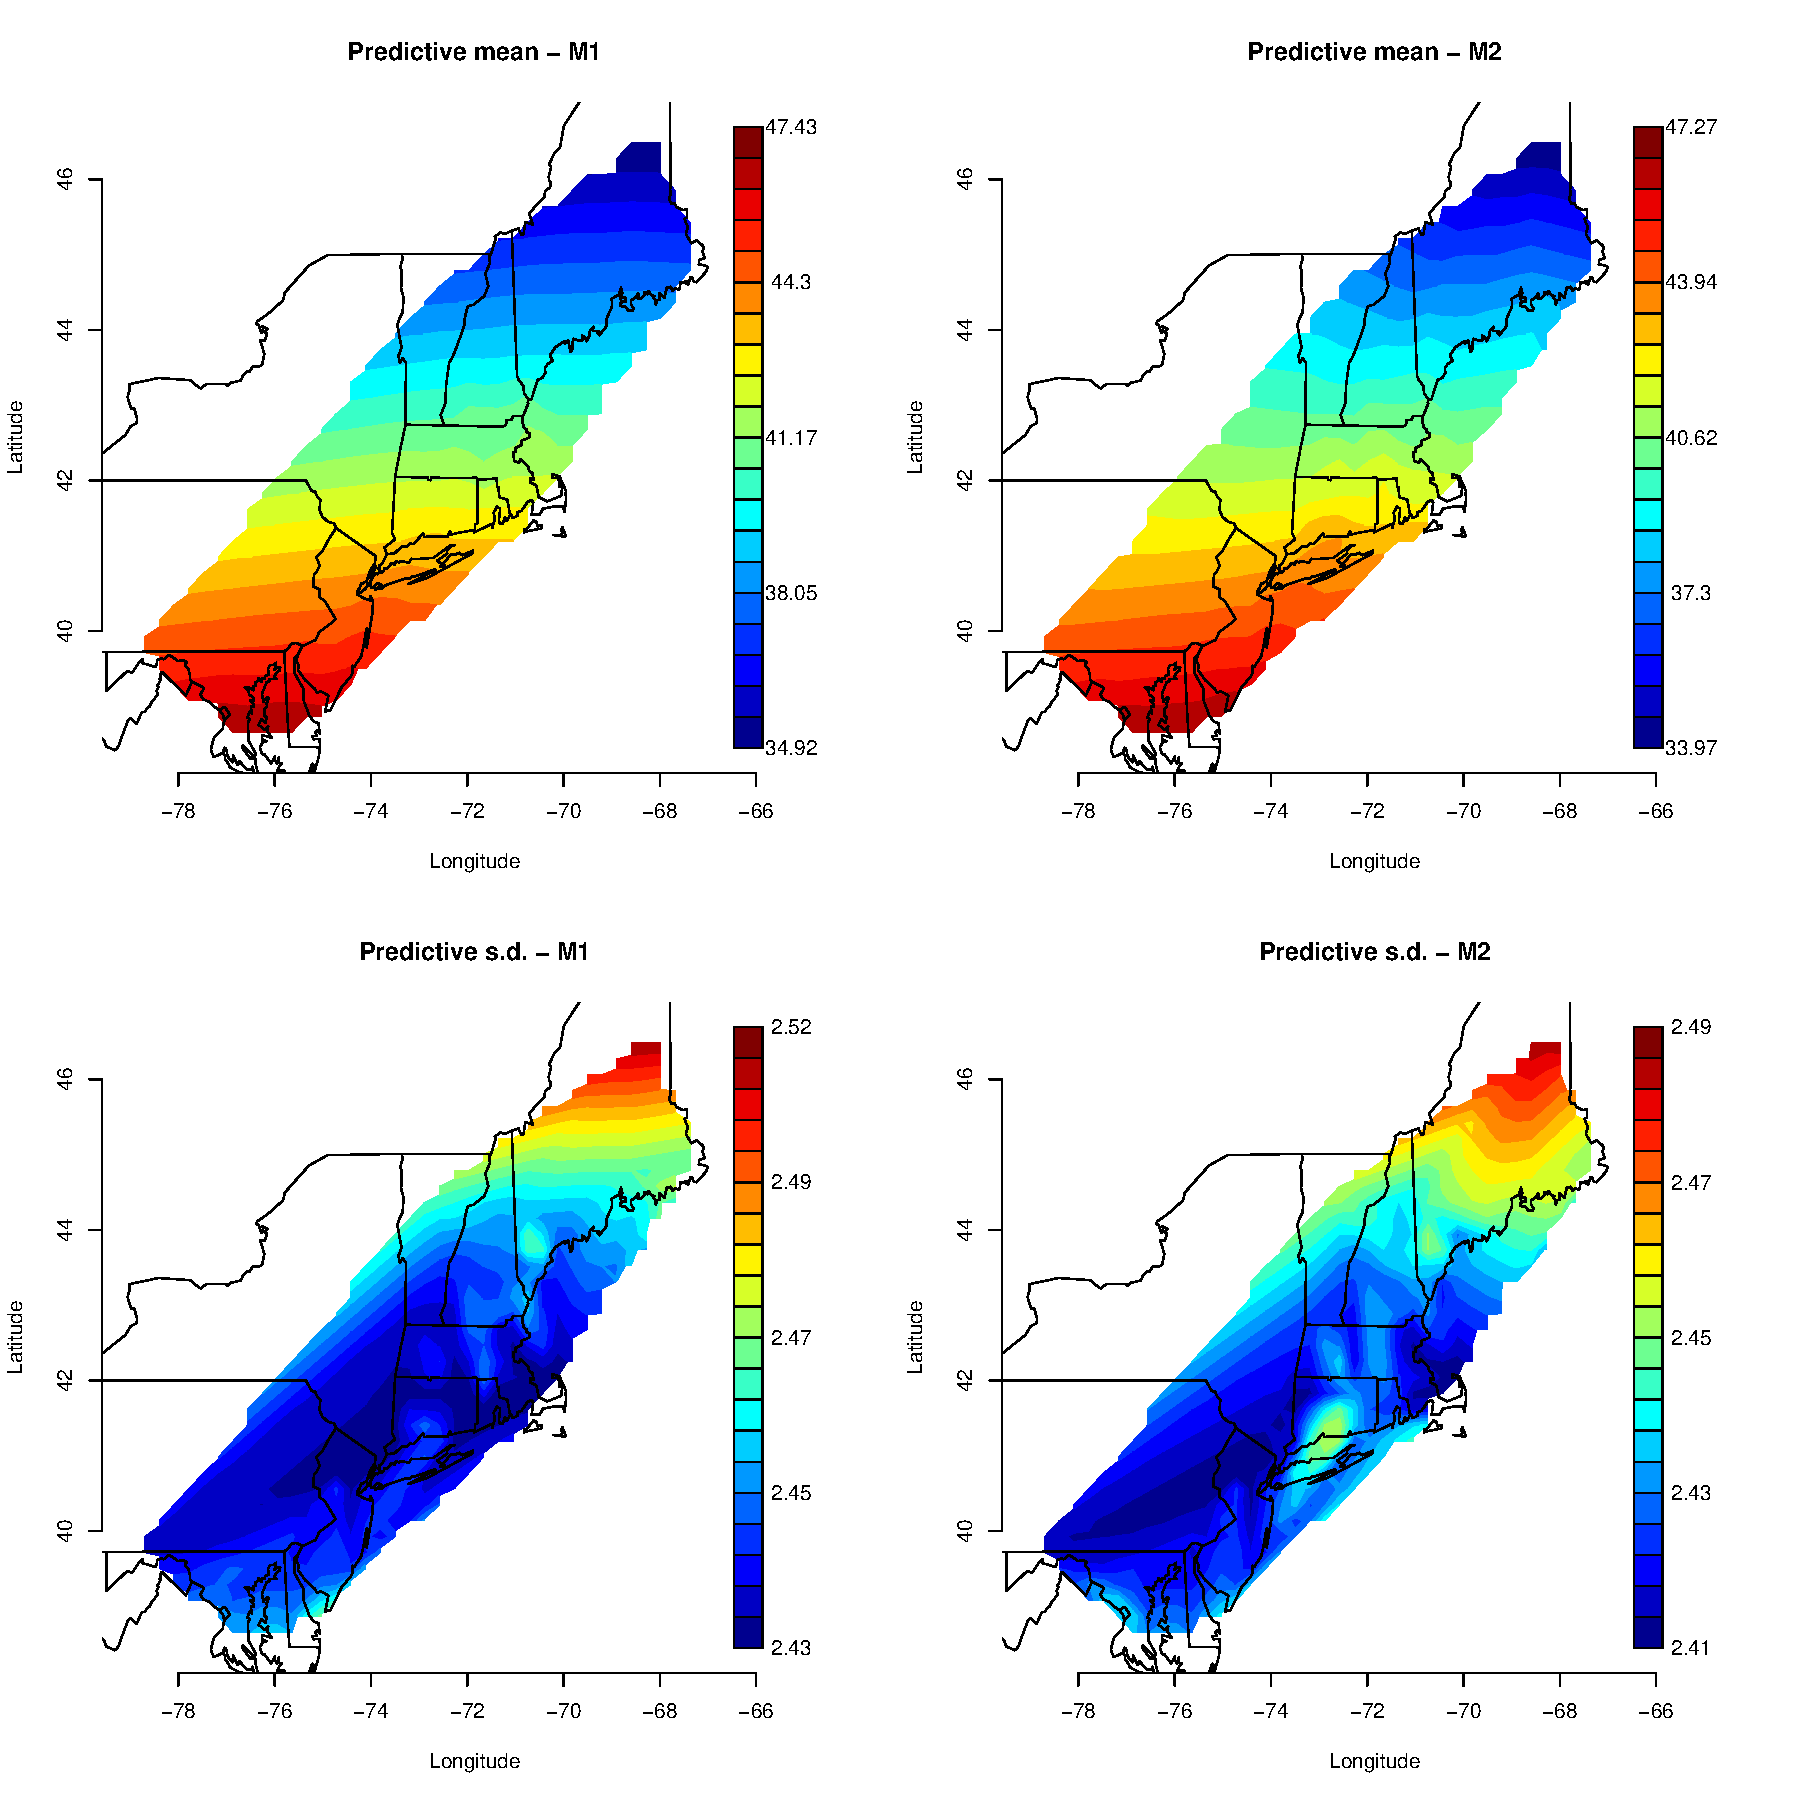
\includegraphics[scale=0.5]{figs/y.pdf}
\end{center}
\caption{Posterior predictive distributions. Top row: mean. Bottom: standard deviation. Left: model 1. Right: model 2.}
\end{figure}

% \begin{figure}[ht]
% \begin{center}
% 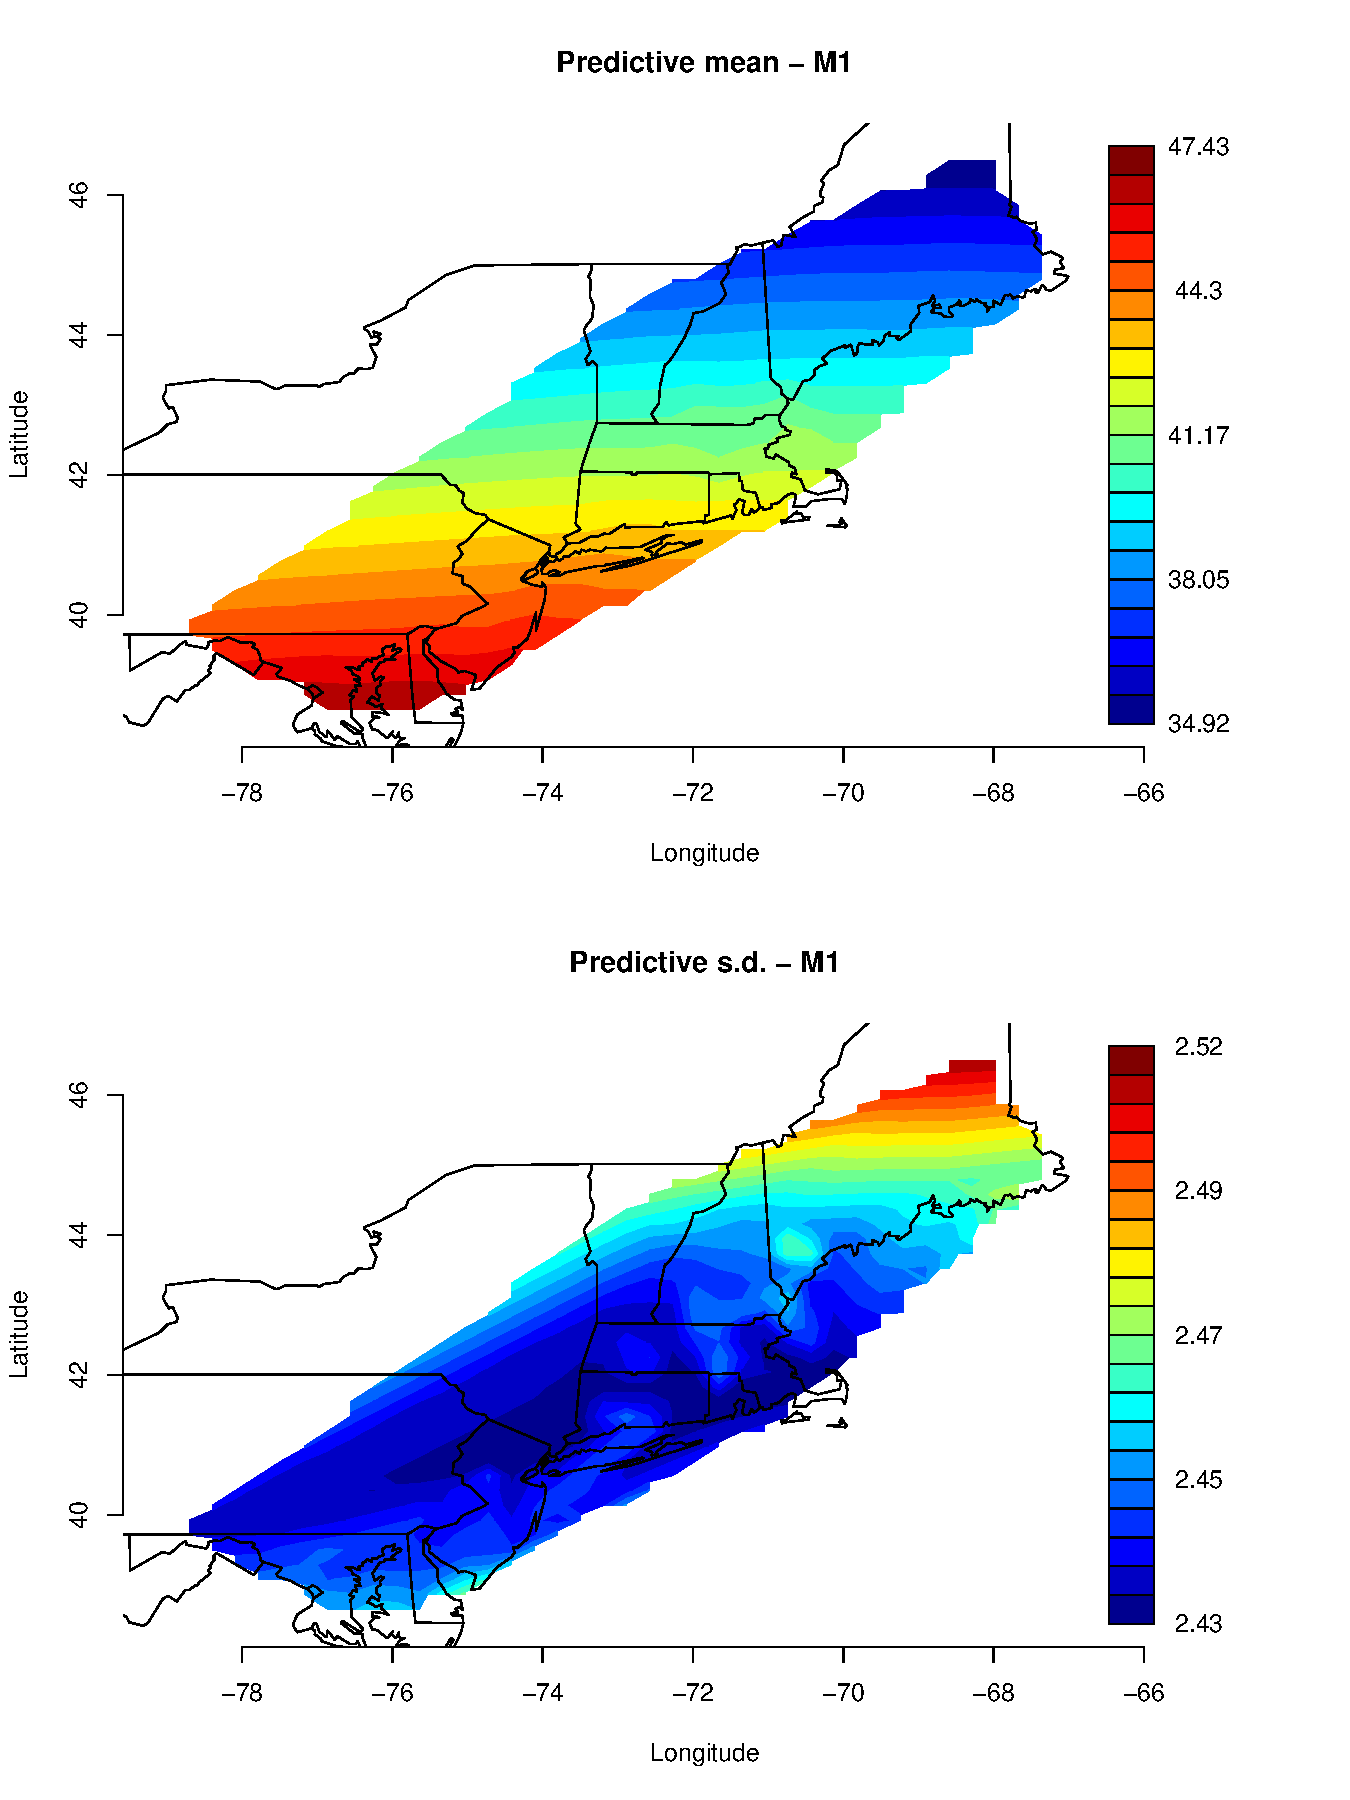
\includegraphics[scale=0.5]{figs/y1.pdf}
% \end{center}
% \caption{Posterior predictive mean and s.d. for model 1}
% \end{figure}
% 
% \begin{figure}[ht]
% \begin{center}
% 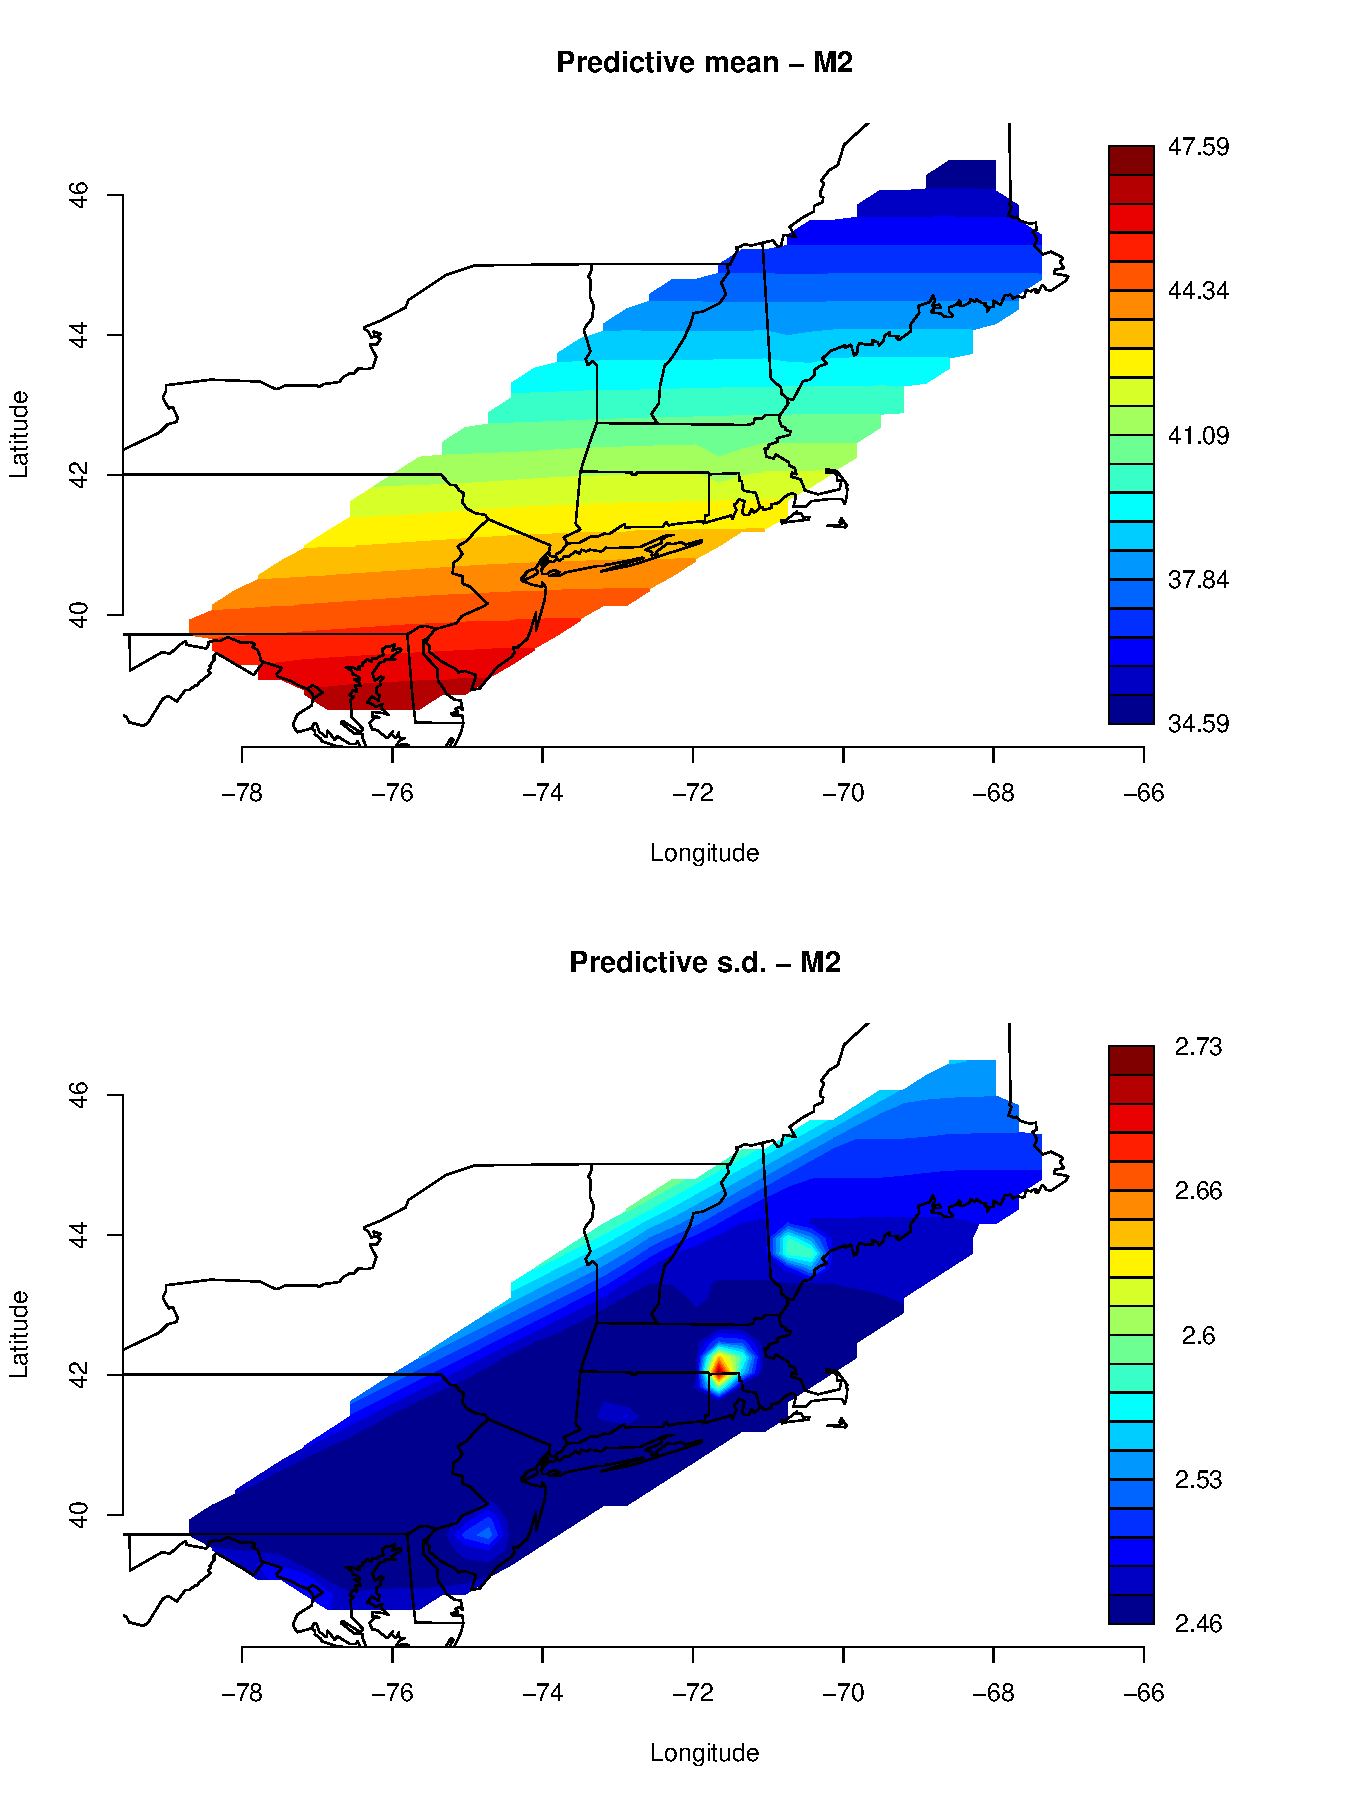
\includegraphics[scale=0.5]{figs/y2.pdf}
% \end{center}
% \caption{Posterior predictive mean and s.d. for model 2}
% \end{figure}

\begin{figure}[ht]
\begin{center}
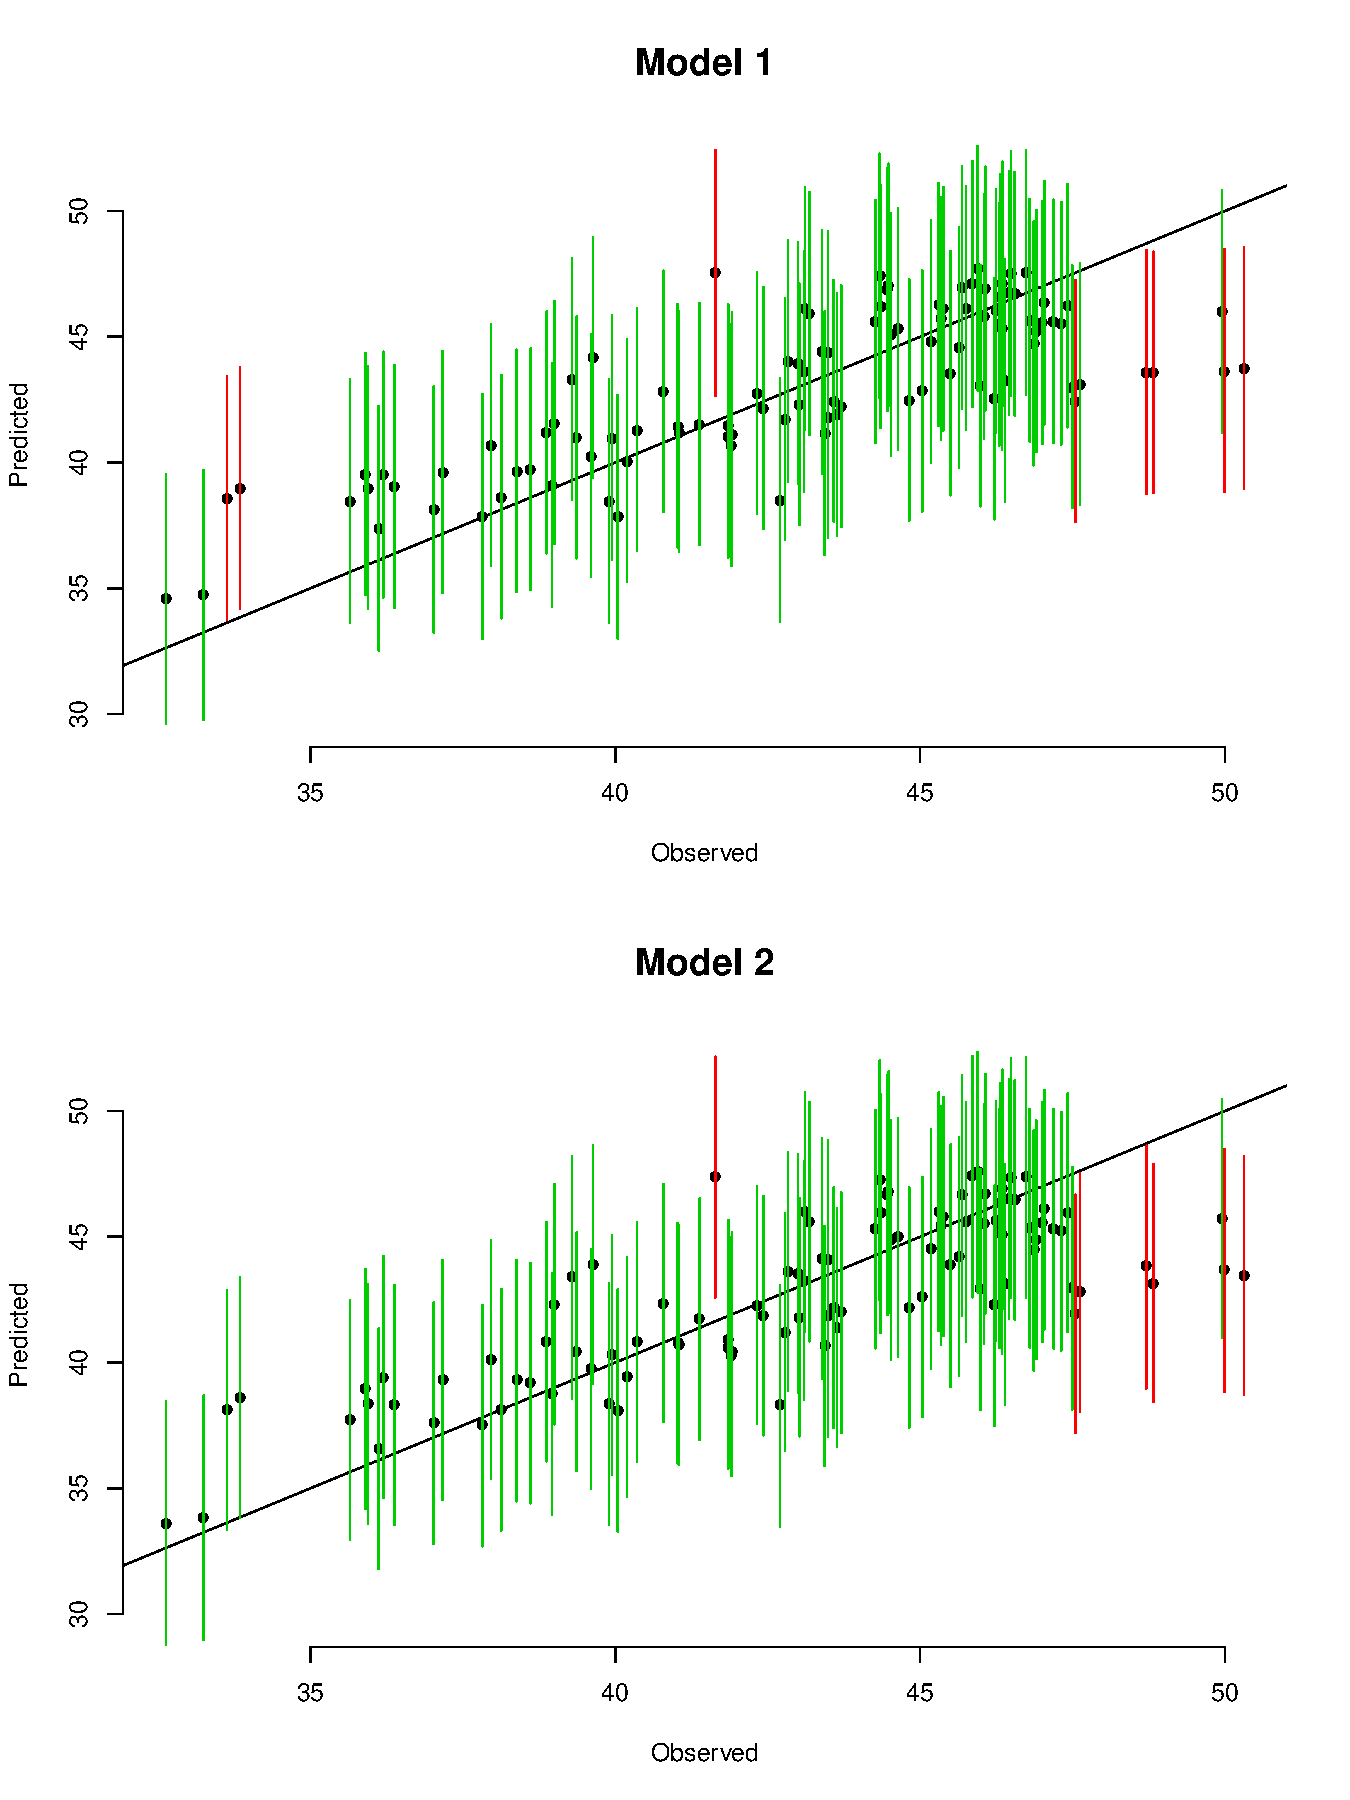
\includegraphics[scale=0.5]{figs/fit.pdf}
\end{center}
\caption{Observed versus fitted plots for models 1 and 2, each with coverage near 0.93}
\end{figure}





\end{document}
